In this lecture, we state and prove Markov's inequality and Chebyshev's inequality, and we state the
Chernoff bound. We then look at the query complexity of search for classical and quantum algorithms,
and we analyze the birthday paradox.

\section{Markov's Inequality}

Markov's inequality uses only the expectation $\expectation{X}$ of the random variable, which is
also called the \emph{first moment}.

\begin{theorem}[Markov's Inequality]\label{thm:markov}
    Let $X \geq 0$ be a random variable. Then, for any $a > 0$,
    \[\prob{X \geq a \expectation{X}} \leq \frac{1}{a}.\]
    Equivalently, for any $b > 0$,
    \[\prob{X \geq b} \leq \frac{\expectation{X}}{b}.\]
\end{theorem}

\begin{figure}[ht]
    \centering
    \begin{tikzpicture}
        \draw (0,0) -- (8,0);
        \draw (0,0.1) -- (0,-0.1) node[below] {\small $0$};
        \draw (3,0.1) -- (3,-0.1);
        \node[above] at (3,0.1) {\small $\mu = \expectation{X}$};
        \draw (6,0.1) -- (6,-0.1) node[below] {\small $a\mu$};
        \draw[decorate, decoration={brace, amplitude=5pt}] (6,0.25) -- (8,0.25)
        node[midway, above=6pt] {\small $\leq \frac{1}{a}$};
    \end{tikzpicture}
    \caption{Markov's inequality: the probability that $X$ is at least $a\mu$ is at most $\sfrac{1}{a}$.}
    \label{fig:markov}
\end{figure}

\begin{proof}
    Let
    \[I = \begin{cases}
            1 & \text{if } X \geq b, \\
            0 & \text{otherwise.}
        \end{cases}\]
    Then
    \[I \leq \frac{X}{b}.\]
    This is true for $X \geq b$, since then $I = 1 \leq \frac{X}{b}$. It is also true for $X < b$,
    since then $I = 0$ and $X \geq 0$.
    Markov's inequality follows by taking expectations on both sides:
    \[\expectation{I} \leq \expectation{\frac{X}{b}} = \frac{\expectation{X}}{b}.\]
    Since
    \[\prob{I = 1} = \prob{X \geq b} \qquad\text{and}\qquad \prob{I = 0} = \prob{X < b},\]
    we have $\expectation{I} = \prob{I = 1}$, and hence
    \[\prob{X \geq b} \leq \frac{\expectation{X}}{b}.\]
    Taking $b = a \expectation{X}$ gives $\prob{X \geq a \expectation{X}} \leq \frac{1}{a}$.
\end{proof}

\section{Chebyshev's Inequality}

Chebyshev's inequality uses the variance of the random variable, which is also called the
\emph{second moment}.

\begin{definition}[Variance and Standard Deviation]
    The \textbf{variance} of a random variable $X$ is
    \[\variance{X} = \expectation{\left(X - \expectation{X}\right)^2}.\]
    The \textbf{standard deviation} of $X$ is
    \[\sigma = \sqrt{\variance{X}}.\]
\end{definition}

\begin{theorem}[Chebyshev's Inequality]\label{thm:chebyshev}
    For any random variable $X$ and any $a > 0$,
    \[\prob{\abs{X - \expectation{X}} \geq a} \leq \frac{\variance{X}}{a^2} = \frac{\sigma^2}{a^2}.\]
\end{theorem}

Here $\abs{X - \expectation{X}}$ is the deviation of $X$ from its mean.

\begin{proof}
    \[\prob{\abs{X - \expectation{X}} \geq a}
        = \prob{\left(X - \expectation{X}\right)^2 \geq a^2}
        \leq \frac{\expectation{\left(X - \expectation{X}\right)^2}}{a^2}
        = \frac{\variance{X}}{a^2},\]
    where the inequality is Markov's inequality applied to the random variable
    $\left(X - \expectation{X}\right)^2 \geq 0$.
\end{proof}

\section{Chernoff Bound}

The Chernoff bounds of the last lecture (\cref{thm:chernoff-0901}) were restated in class with the
independence assumption made explicit. For a sum $X = \sum_{i=1}^{n} X_i$ of \emph{mutually
independent} indicator random variables with $\prob{X_i = 1} = p_i$, linearity of expectation gives
$\mu = \expectation{X} = \sum_{i=1}^{n} p_i$, and for $0 < \delta < 1$
\[\prob{X \geq (1+\delta)\mu} \leq e^{-\frac{\mu \delta^2}{3}},
    \qquad
    \prob{X < (1-\delta)\mu} \leq e^{-\frac{\mu \delta^2}{2}},\]
and $\prob{X \geq R} \leq 2^{-R}$ for $R \geq 6\mu$.

\section{Search}

Let $f \colon D \to R$ be a function from a domain $D$ to a range $R$ (\cref{fig:function}).
Given $y$, we ask: is there an $x$ such that $f(x) = y$? We consider
\[f \colon [1, \dots, N] \to [1, \dots, N],\]
and we want to find an $x$ such that $f(x) = k$. The function can be seen as an array with $n$
slots, where $n$ is the size of the domain, and the cost of an algorithm is the number of queries
to $f$.

\begin{figure}[ht]
    \centering
    \begin{tikzpicture}
        % array
        \draw (0,0) rectangle (6,0.7);
        \foreach \x in {1,2,4,5} {\draw (\x,0) -- (\x,0.7);}
        \node at (3,0.35) {$\cdots$};
        \node[below] at (0.5,0) {\small $1$};
        \node[below] at (5.5,0) {\small $n$};
        % function from D to R
        \draw (8.5,0.35) ellipse (0.6 and 1);
        \draw (11.5,0.35) ellipse (0.6 and 1);
        \node at (8.5,1.65) {$D$};
        \node at (11.5,1.65) {$R$};
        \node[point] (y) at (11.5,0.35) {};
        \foreach \h in {0.95,0.35,-0.25} {
                \node[point] (x) at (8.5,\h) {};
                \draw[->] (x) -- (y);
            }
        \node at (10,1.35) {$f$};
    \end{tikzpicture}
    \caption{Left: an array with $n$ slots. Right: a function $f \colon D \to R$.}
    \label{fig:function}
\end{figure}

\begin{itemize}
    \item Randomized classical algorithm: $\bigTh{n}$ queries.
    \item Grover's algorithm: $\bigO{\sqrt{n}}$ queries.
\end{itemize}

For the random sampling algorithm,
\[\expectation{\text{queries}} = \bigO{n}, \qquad \prob{\text{Success}} = \frac{1}{n}.\]

\paragraph{Probability amplitude amplification.} If the classical success probability is $p$, then
in the quantum case it becomes $\sqrt{p}$.

\section{Birthday Paradox}

There are $m$ people and $n$ birthdays ($n = 365$). We are looking for a \emph{collision}, i.e.,
$x \neq y$ such that
\[f(x) = f(y),\]
where $f(x)$ is the birthday of person $x$.

Let $E_i$ be the event that the $\nth{i}$ birthday is different from the first $i-1$ birthdays. Then
\begin{align*}
    \prob{\bigcap_{i=1}^{m} E_i}
     & = \prob{\text{all birthdays different}}                                                                        \\
     & = \prob{E_1} \cdot \prob{E_2 \given E_1} \cdot \prob{E_3 \given E_2 \cap E_1} \cdots                           \\
     & = 1 \cdot \left(1 - \frac{1}{n}\right) \cdot \left(1 - \frac{2}{n}\right) \cdots \left(1 - \frac{m-1}{n}\right) \\
     & = \prod_{i=0}^{m-1} \left(1 - \frac{i}{n}\right)                                                                \\
     & \leq \prod_{i=0}^{m-1} e^{-\sfrac{i}{n}}                                                                        \\
     & = e^{-\sum_{i=0}^{m-1} \frac{i}{n}}                                                                             \\
     & = e^{-\frac{(m-1)m}{2n}}.
\end{align*}
For $m = \sqrt{2n} + 1$,
\[\prob{\text{all birthdays different}}
    \leq e^{-\frac{\sqrt{2n}\left(\sqrt{2n}+1\right)}{2n}}
    \leq e^{-\frac{2n}{2n}}
    = \frac{1}{e}
    \leq \frac{1}{2}.\]
Hence $\bigO{\sqrt{n}}$ people are enough to have a constant probability of collision.

\subsection{Expected Number of Collisions}

The birthday paradox can be seen as throwing $m$ balls into $n$ bins (\cref{fig:ballsbins}).
We show that for $m \approx \sqrt{2n}$,
\[\expectation{\text{\# collisions}} \geq 1.\]

\begin{figure}[ht]
    \centering
    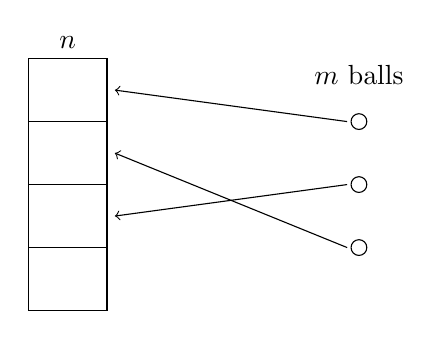
\begin{tikzpicture}
        % bins
        \draw (0,0) rectangle (1,3.2);
        \foreach \y in {0.8,1.6,2.4} {\draw (0,\y) -- (1,\y);}
        \node[above] at (0.5,3.2) {$n$};
        % balls
        \node[above] at (4.2,2.75) {$m$ balls};
        \foreach \b/\t in {2.4/2.8, 1.6/1.2, 0.8/2.0} {
                \draw (4.2,\b) circle (0.1);
                \draw[->] (4.05,\b) -- (1.1,\t);
            }
    \end{tikzpicture}
    \caption{$m$ balls are thrown into $n$ bins.}
    \label{fig:ballsbins}
\end{figure}

Let $X$ be the number of collisions. $X$ takes values from $0$ to $\binom{m}{2}$. Write
\[X = \sum_{i \neq j} X_{ij},
    \qquad
    X_{ij} = \begin{cases}
        1 & \text{if } f(i) = f(j), \\
        0 & \text{else,}
    \end{cases}\]
where the sum is over the $\binom{m}{2}$ pairs $i \neq j$. The random variables $X_{ij}$ are
\emph{pairwise independent}. By linearity of expectation,
\begin{align*}
    \expectation{X}
     & = \sum_{i \neq j} \expectation{X_{ij}} \\
     & = \sum_{i \neq j} \prob{X_{ij} = 1}    \\
     & = \sum_{i \neq j} \frac{1}{n}          \\
     & = \binom{m}{2} \frac{1}{n}
    = \frac{m(m-1)}{2n}
    \sim \frac{m^2}{2n}
    = \bigTh{\frac{m^2}{n}}.
\end{align*}

% Dashed box in my notes: exercise given in class.
\begin{exercise}\label{ex:birthday-0903}
    Show that
    \[\prob{X \geq 1} \geq \bigTh{1},\]
    i.e., the birthday paradox occurs.
\end{exercise}

The hint given in class is to compute the variance
\[\variance{X} = \variance{\sum_{i \neq j} X_{ij}}\]
and to use Chebyshev's inequality (\cref{thm:chebyshev}): if the variance of $X$ is small compared
to $\expectation{X}^2$, then $X$ is rarely far from its mean, and in particular rarely $0$. We first
prove the claim that the $X_{ij}$ are pairwise independent, which is what makes the variance easy
to compute.

\begin{lemma}[Variance of the Number of Collisions]\label{lem:pairwise-0903}
    For any two different pairs $\set{i,j} \neq \set{k,l}$,
    \[\expectation{X_{ij} X_{kl}} = \expectation{X_{ij}} \expectation{X_{kl}} = \frac{1}{n^2},\]
    i.e., $X_{ij}$ and $X_{kl}$ are independent. Consequently
    \[\variance{X} = \sum_{i \neq j} \variance{X_{ij}}
        = \binom{m}{2} \frac{1}{n} \left(1 - \frac{1}{n}\right) \leq \expectation{X}.\]
\end{lemma}

\begin{proof}
    Since $X_{ij} X_{kl} = 1$ exactly when both indicators are $1$,
    \[\expectation{X_{ij} X_{kl}} = \prob{f(i) = f(j) \text{ and } f(k) = f(l)}.\]
    There are two cases.
    \begin{itemize}
        \item The pairs are disjoint, $\set{i,j} \cap \set{k,l} = \emptyset$. Then the two events
              depend on the birthdays of four different people, which are independent, so the
              probability is $\prob{f(i) = f(j)} \cdot \prob{f(k) = f(l)} = \sfrac{1}{n^2}$.
        \item The pairs share one person, say $\set{i,j}$ and $\set{i,k}$ with $j \neq k$. The
              birthdays $f(j)$ and $f(k)$ are independent of $f(i)$ and of each other, and each
              equals a given day $b$ with probability $\sfrac{1}{n}$, so
              \[\prob{f(j) = f(i) \text{ and } f(k) = f(i)}
                  = \sum_{b=1}^{n} \prob{f(i) = b} \cdot \frac{1}{n} \cdot \frac{1}{n}
                  = \frac{1}{n^2}.\]
    \end{itemize}
    In both cases $\expectation{X_{ij} X_{kl}} = \sfrac{1}{n^2} = \expectation{X_{ij}} \expectation{X_{kl}}$.
    For two indicator random variables this is the same as independence, since their joint
    distribution is determined by $\prob{X_{ij} = 1}$, $\prob{X_{kl} = 1}$ and $\prob{X_{ij} = X_{kl} = 1}$.

    For the variance, write $X - \expectation{X} = \sum_{i \neq j} \left(X_{ij} - \expectation{X_{ij}}\right)$
    and expand the square:
    \begin{align*}
        \variance{X}
         & = \expectation{\Big(\sum_{i \neq j} \left(X_{ij} - \expectation{X_{ij}}\right)\Big)^2}                                                           \\
         & = \sum_{i \neq j} \expectation{\left(X_{ij} - \expectation{X_{ij}}\right)^2}
        + \sum_{\set{i,j} \neq \set{k,l}} \expectation{\left(X_{ij} - \expectation{X_{ij}}\right) \left(X_{kl} - \expectation{X_{kl}}\right)} \\
         & = \sum_{i \neq j} \variance{X_{ij}}
        + \sum_{\set{i,j} \neq \set{k,l}} \left(\expectation{X_{ij} X_{kl}} - \expectation{X_{ij}} \expectation{X_{kl}}\right)
        = \sum_{i \neq j} \variance{X_{ij}},
    \end{align*}
    where the second sum vanishes by the first part. Finally $X_{ij}$ is an indicator with
    $\prob{X_{ij} = 1} = \sfrac{1}{n}$, so $X_{ij}^2 = X_{ij}$ and
    \[\variance{X_{ij}} = \expectation{X_{ij}^2} - \expectation{X_{ij}}^2
        = \frac{1}{n} - \frac{1}{n^2} = \frac{1}{n} \left(1 - \frac{1}{n}\right) \leq \frac{1}{n}.\]
    Summing over the $\binom{m}{2}$ pairs gives $\variance{X} \leq \binom{m}{2} \frac{1}{n} = \expectation{X}$.
\end{proof}

\begin{theorem}[The Birthday Paradox Occurs]\label{thm:birthday-0903}
    If $m \geq 2\sqrt{n} + 1$, then
    \[\prob{X \geq 1} \geq \frac{1}{2}.\]
    In words: with $\bigO{\sqrt{n}}$ people there is a collision with constant probability.
\end{theorem}

\begin{proof}
    The event $X = 0$ (no collision) is contained in the event $\abs{X - \expectation{X}} \geq \expectation{X}$,
    since $X = 0$ means $X - \expectation{X} = -\expectation{X}$. By Chebyshev's inequality
    (\cref{thm:chebyshev}) with $a = \expectation{X}$, and then \cref{lem:pairwise-0903},
    \[\prob{X = 0} \leq \prob{\abs{X - \expectation{X}} \geq \expectation{X}}
        \leq \frac{\variance{X}}{\expectation{X}^2} \leq \frac{\expectation{X}}{\expectation{X}^2} = \frac{1}{\expectation{X}}.\]
    For $m \geq 2\sqrt{n} + 1$, since $m(m-1)$ grows with $m$,
    \[\expectation{X} = \frac{m(m-1)}{2n} \geq \frac{(2\sqrt{n} + 1) \cdot 2\sqrt{n}}{2n}
        = \frac{4n + 2\sqrt{n}}{2n} \geq 2,\]
    so $\prob{X = 0} \leq \sfrac{1}{2}$, and $\prob{X \geq 1} = 1 - \prob{X = 0} \geq \sfrac{1}{2}$.
\end{proof}

The direct computation of $\prob{\text{all birthdays different}}$ above already gave
$\prob{X = 0} \leq \sfrac{1}{e}$ for $m = \sqrt{2n} + 1$. The point of this \emph{second moment}
argument is that it only uses $\expectation{X}$ and $\variance{X}$, so it also works when the exact
probability cannot be computed.

\section{Quantum Birthday Paradox}

The birthday paradox, seen as an algorithm, solves the \emph{collision problem}: given query access
to a function $f$, find $x \neq y$ with $f(x) = f(y)$. Querying $m = \sqrt{2n} + 1$ random points finds
a collision with probability at least $\sfrac{1}{2}$, so $\bigO{\sqrt{n}}$ queries suffice classically.
The quantum version of the problem is studied later in the course; here we show that classically
$\sqrt{n}$ queries are also necessary. An algorithm makes $k$ queries
\[f(x_1), \dots, f(x_k),\]
where the point $x_s$ may depend on the earlier answers $f(x_1), \dots, f(x_{s-1})$ and on random coins.

% Not in a dashed box in my notes, but written as something to show.
\begin{exercise}\label{ex:collision-lb-0903}
    Show a $\sqrt{n}$ lower bound in the classical case.
\end{exercise}

We use the same model as in the birthday paradox: $f \colon D \to [n]$, where $[n] = \set{1, \dots, n}$,
is a \emph{random function}, i.e., every value $f(x)$ is uniform in $[n]$ and independent of all the
other values (the birthday of person $x$). The algorithm \emph{finds a collision} if it outputs
$x \neq y$ with $f(x) = f(y)$. We may assume that the algorithm queries the two points that it
outputs: if it does not, it can do so with at most $2$ extra queries, which does not change the
bound below. We may also assume that the $k$ queried points are different, since repeating a query
gives no new information.

\begin{theorem}[Classical Lower Bound for Collision Finding]\label{thm:collision-lb-0903}
    Let $f \colon D \to [n]$ be a random function. Every classical algorithm (deterministic or
    randomized, adaptive) that makes $k$ queries finds a collision with probability at most
    \[\frac{\binom{k}{2}}{n} = \frac{k(k-1)}{2n}.\]
    In particular, to find a collision with probability at least $\sfrac{1}{2}$ it needs
    $k > \sqrt{n}$ queries, so the classical query complexity of the collision problem is $\bigOm{\sqrt{n}}$.
\end{theorem}

\begin{proof}
    Since the algorithm queries the points that it outputs, it can only find a collision if two of
    its queried values agree. Let $E_s$ be the event that the $\nth{s}$ query collides with an earlier
    one, i.e., $f(x_s) \in \set{f(x_1), \dots, f(x_{s-1})}$. A collision among the $k$ queries means
    that some $E_s$ occurs, so by the union bound
    \[\prob{\text{collision}} \leq \sum_{s=1}^{k} \prob{E_s}.\]
    We claim that $\prob{E_s} \leq \frac{s-1}{n}$. Consider the moment just before the $\nth{s}$
    query. The algorithm chooses $x_s$ from the $s-1$ answers seen so far and from its random coins;
    condition on all of these. Then $x_s$ is a fixed point that has not been queried before, so its
    value $f(x_s)$ is still a uniformly random element of $[n]$, independent of the $s-1$ values
    $f(x_1), \dots, f(x_{s-1})$, which are now fixed. The probability that $f(x_s)$ equals one of these
    $s-1$ fixed values is therefore at most $\frac{s-1}{n}$, no matter how the algorithm chose $x_s$.
    Since this holds for every outcome of the first $s-1$ steps, it also holds without conditioning,
    which proves the claim. Hence
    \[\prob{\text{collision}} \leq \sum_{s=1}^{k} \frac{s-1}{n} = \frac{0 + 1 + \dots + (k-1)}{n} = \frac{k(k-1)}{2n}.\]
    If the algorithm succeeds with probability at least $\sfrac{1}{2}$, then $\frac{k(k-1)}{2n} \geq \frac{1}{2}$,
    i.e., $k^2 > k(k-1) \geq n$, so $k > \sqrt{n}$.
\end{proof}

\paragraph{Worst case inputs.} \cref{thm:collision-lb-0903} is a statement about a \emph{random}
input $f$: the distributional complexity of the collision problem under the uniform distribution on
functions is $\bigOm{\sqrt{n}}$. By Yao's minmax principle from the lecture of September~1 (in its
version for algorithms that are allowed to err), this is also a lower bound for every randomized
algorithm on its worst case input. Together with the birthday paradox, which finds a collision with
$\bigO{\sqrt{n}}$ queries, the classical query complexity of finding a collision is $\bigTh{\sqrt{n}}$.
